% CVPR 2023 Paper Template
% based on the CVPR template provided by Ming-Ming Cheng (https://github.com/MCG-NKU/CVPR_Template)
% modified and extended by Stefan Roth (stefan.roth@NOSPAMtu-darmstadt.de)

\documentclass[10pt,twocolumn,letterpaper]{article}

%%%%%%%%% PAPER TYPE  - PLEASE UPDATE FOR FINAL VERSION
\usepackage{cvpr}      % To produce the REVIEW version

% Include other packages here, before hyperref.
\usepackage{graphicx}
\usepackage{amsmath}
\usepackage{amssymb}
\usepackage{booktabs}
\usepackage{subcaption}

% It is strongly recommended to use hyperref, especially for the review version.
% hyperref with option pagebackref eases the reviewers' job.
% Please disable hyperref *only* if you encounter grave issues, e.g. with the
% file validation for the camera-ready version.
%
% If you comment hyperref and then uncomment it, you should delete
% ReviewTempalte.aux before re-running LaTeX.
% (Or just hit 'q' on the first LaTeX run, let it finish, and you
%  should be clear).
\usepackage[pagebackref,breaklinks,colorlinks]{hyperref}

% Support for easy cross-referencing
\usepackage[capitalize]{cleveref}
\crefname{section}{Sec.}{Secs.}
\Crefname{section}{Section}{Sections}
\Crefname{table}{Table}{Tables}
\crefname{table}{Tab.}{Tabs.}

%%%%%%%%% PAPER ID  - PLEASE UPDATE
\def\cvprPaperID{*****} % *** Enter the CVPR Paper ID here
\def\confName{CVPR}
\def\confYear{2023}

\begin{document}

\newcommand{\dhimitrios}[1]{\textcolor{red}{Dhimitrios: #1}}

%%%%%%%%% TITLE - PLEASE UPDATE
\title{Team \#16: From Strings to Sequences --- Classifying and Generating Music from Acoustic Guitar Notes}


\author{
  Camilo Martínez\\
  7057573\\
  \and
  Dhimitrios Duka\\
  7059153\\
  \and
  Honglu Ma\\
  7055053\\
}
\maketitle

%%%%%%%%% BODY TEXT
\section{Abstract}
% Should be inside \emph{} https://openaccess.thecvf.com/content/CVPR2022W/WMF/papers/Guarnera_On_the_Exploitation_of_Deepfake_Model_Recognition_CVPRW_2022_paper.pdf
\emph{Lorem ipsum dolor sit amet, consectetur adipiscing elit}

\section{Introduction}

\section{Related Work}  

\section{Method}

\subsection{Datasets}
\dhimitrios{Not sure if Datasets should be under methods}

We identified a significant gap in available datasets for the task of guitar chord recognition, which made us create our own. We recorded 90-second videos for each chord in three different environments, ensuring high quality by capturing them in 4K resolution at 60 frames per second. From these videos, we extracted frames and downsampled them to a resolution of 640 $\times$ 360 pixels. This process generated approximately 30,000 frames per chord.

\begin{figure}[h]
  \centering
  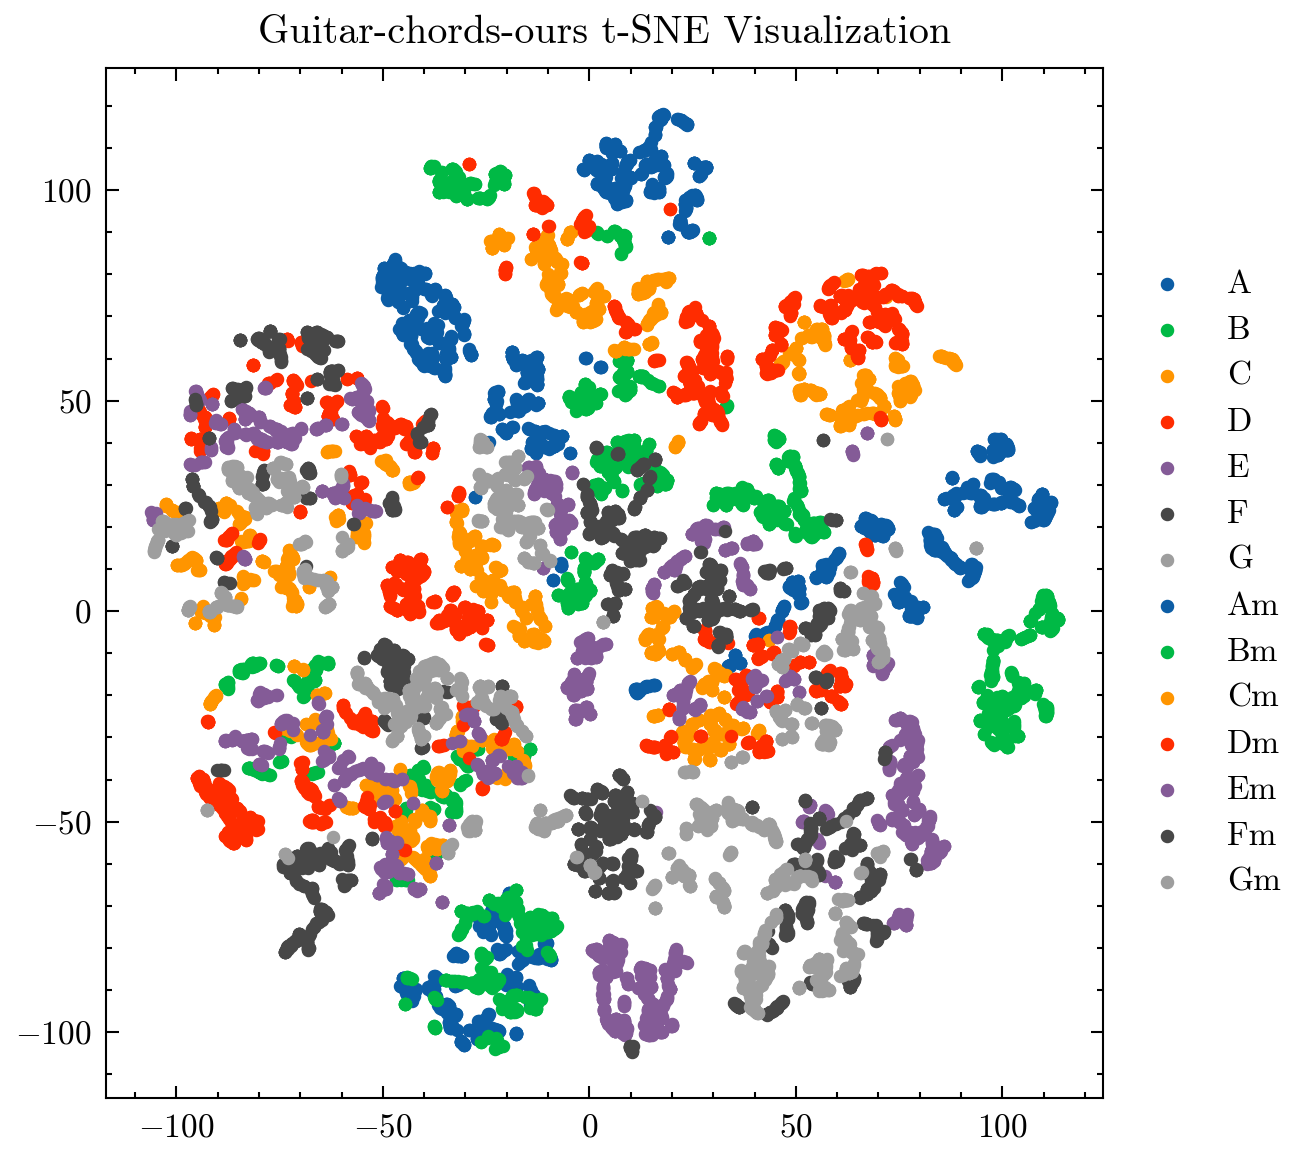
\includegraphics[width=0.3\textwidth]{images/final/Guitar-chords-ours_tsne_plot.png}
  \caption{The t-SNE plot of our dataset containing 14 chords. Each point represents a KNN-sampled frame, with the color indicating the corresponding chord label.}
  \label{fig:ours-tsne-plot}
\end{figure}

To reduce redundancy, we limit the dataset to 1,000 frames for each of the 14 chords. To increase the diversity of the dataset, we used two different sampling methods: simple random sampling and KNN-based sampling. In the former method, we selected 1,000 frames at random while in the latter, we used the KNN algorithm to choose 1,000 frames that were the most distinct from one another.

Unfortunately, both sampling strategies resulted in an overly simplistic dataset that failed to capture the real-world complexity of chords, as shown by Figure \ref{fig:ours-tsne-plot}. This resulted in poor model generalization. However, rather than abandoning our dataset, \textbf{Guitrar\_chords\_ours}, we used it as a test set to evaluate the generalizability of our model. In the end, we decided to use existing datasets \cite{guitar-chord-tvon8_dataset,guitar-chord-bounding-box_dataset, guitar-chord-handshape_dataset, guitar-chords-daewp_dataset} for training the models, merging them to create a more complex dataset, \textbf{Guitar\_chords}, which resulted in significantly better results.

This change in our approach necessitated a change in the scope of our chord recognition task. As a consequence of using existing datasets, we were limited to only seven chords in total—A, B, C, D, E, F, and G—down from the 14 chords originally planned.

\section{Experimental Results and Analyses}
\label{sec:results}

\subsection{Guitar Chord Classification}
To evaluate our approaches against those in the original paper, we implemented the InceptionResNetv2 model as described by the authors. After training the model on our datasets, we obtained the results shown in Table \ref{tab:handpose-classifier-results}, which provided us with a baseline to compare our models against.

\subsubsection{Hand Pose Estimation + Classifier}
First, we wanted to try a simple yet interesting approach. For a given sample image $\zeta$, we utilized a hand pose estimation model to extract the hand shape from it, which was then used as the input to a classifier.

\begin{figure}[h]
  \centering
  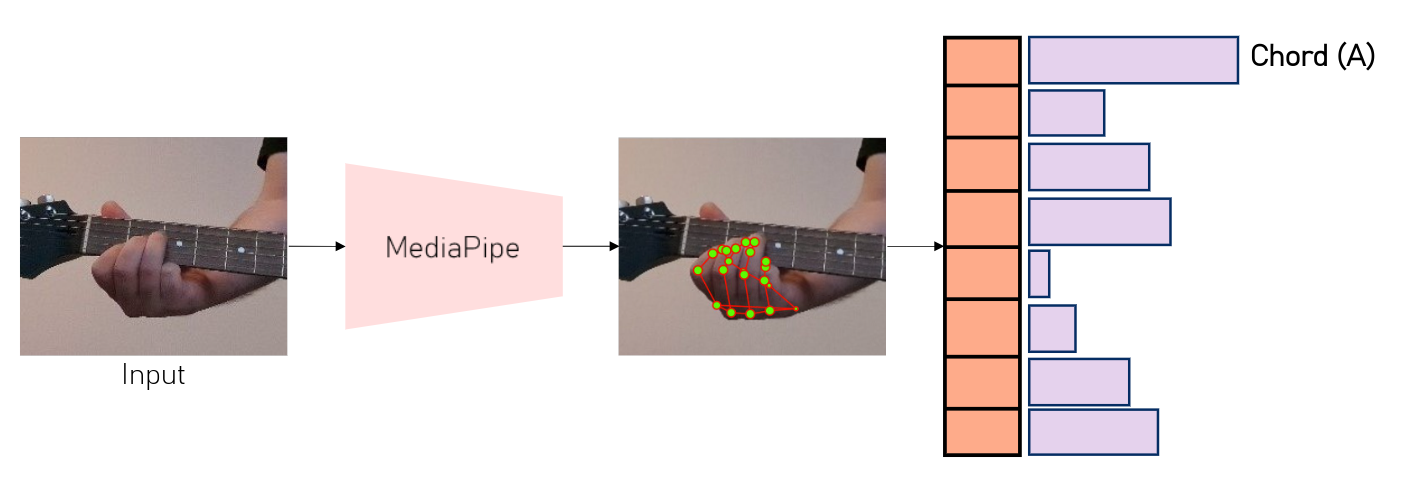
\includegraphics[width=0.5\textwidth]{images/final/hand_pose_estimation_classifier.png}
  \caption{t-SNE plot of our dataset. Each point represents a sampled frame, and the color indicates the chord label. }
  \label{fig:ours-tsne-plot}
\end{figure}

We used MediaPipe \cite{zhang2020mediapipe} to extract the hand shape followed by different classifiers—SVM, Random Forest, and a simple MLP—to classify the chords. The results of this approach are summarized in Table \ref{tab:handpose-classifier-results}.

Surprisingly, this approach performed well, achieving good accuracy during validation and testing on two datasets. However, the model struggled to generalize to the third dataset, which we created. This outcome was anticipated, as the samples in our dataset were out of distribution, and the model lacked the complexity needed to generalize effectively to such data.

\dhimitrios{Should we point out that Hand Pose Estimation + Classifier performed better than InceptionResNetv2?}

\begin{table}[h]
  \centering
  \begin{tabular}{lccc}
    \toprule
    \textbf{Model} & \textbf{GC} & \textbf{GCT} & \textbf{GCO} \\
    \midrule
 InceptionResNetv2 & 83.56\% & 68.63\% & 15.57\% \\
    \midrule
 SVM & 95.27\% & 85.71\% & 18.61\% \\
 Random Forest & 93.35\% & 52.41\% & 16.16\%  \\
 MLP & 89.44\% & 78.57\% & 14.39\% \\
    \bottomrule
  \end{tabular}
  \caption{Accuracy of the Hand Pose Estimation + Classifier in the test set of different datasets. \textbf{GC}: Guitar\_Chords, \textbf{GCT}: Guitar\_Chords\_Tiny, \textbf{GCO}: Guitar\_Chords\_Ours.}
  \label{tab:handpose-classifier-results}
\end{table}

\subsubsection{Classifier only}
In the previous experiments, we found out that the Hand Pose Estimation + Classifier approach lacked the robustness necessary to generalize effectively to out-of-distribution data. To address this limitation, we decided to explore more complex models, such as Vision Transformers (ViT) \cite{dosovitskiy2020image} and DINOv2 \cite{oquab2023dinov2}. We evaluated various configurations of these models, including ViT-B/16, ViT-B/32, ViT-L/16, ViT-L/32, DINOv2-S, and DINOv2-L. The results of these experiments are summarized in Table \ref{tab:transformer-models-results}.

\begin{table}[h]
  \centering
  \begin{tabular}{lccc}
    \toprule
    \textbf{Model} & \textbf{GC} & \textbf{GCT} & \textbf{GCO} \\
    \midrule
    InceptionResNetv2 & 83.56\% & 68.63\% & 15.57\% \\
    \midrule
    ViT-B/16 & 98.96\% & 85.29\% & 96.24\% \\
    ViT-B/32 & 93.07\% & 81.37\% & 95.83\% \\
    ViT-L/16 & 95.84\% & 81.37\% & 12.29\% \\
    ViT-L/32 & 77.03\% & 43.14\% & 13.43\% \\
    DINOv2-S & 96.24\% & 88.24\% & 98.18\% \\
    DINOv2-L & 96.44\% & 91.18\% & 97.92\% \\
    \bottomrule
  \end{tabular}
  \caption{Accuracy of Classifier only in the test set of different datasets.}
  \label{tab:transformer-models-results}
\end{table}

As can be seen from Table \ref{tab:transformer-models-results}, ViT models show varying performance across different datasets. The base models, ViT-B/16 and ViT-B/32, perform exceptionally well, with high accuracy on all datasets. However, the larger models, ViT-L/16 and ViT-L/32, do not outperform the base models, suggesting that increased model size does not necessarily correlate with improved performance for this particular task. We expect that the larger models are overfitting the data, as they have more parameters to learn from and our data is limited.

We can also see that the patch 16 versions of the ViT models perform better than the patch 32 versions. This is likely due to the fact that the patch 16 versions have a higher resolution, to capture fine details and maintain higher spatial resolution, which is important for accurately distinguishing between chord shapes and hand positions

Both DINOv2 variants, small and large, demonstrated strong and consistent performance across all datasets. The DINOv2-large model, in particular, achieved the highest accuracy (0.979) on the Guitar\_Chords\_Ours dataset, slightly outperforming the small variant.

The superior performance of DINOv2 can be attributed to its self-supervised learning approach. Unlike models pre-trained on ImageNet, which does not contain specific classes related to 'hands,' DINOv2's self-supervised learning allows it to develop more general and transferable representations, leading to better generalization in our specific task. This enhanced generalization is further supported by attention visualizations of the model when applied to images from the 'ours' dataset, where the model correctly focuses on the hand performing the fretting.

\section{Conclusion}

\section{Discussion}
Currently, we are missing a background class in the dataset.


 %%%%%%%%% REFERENCES
 {\small
  \bibliographystyle{ieee_fullname}
  \bibliography{references}
 }

\end{document}